%%%%%%%%%%%%%%%%%%%%%%%%%%%%%%%%%%%%%%%%%%%%%%%%%%%%%%%%%%%%%%%%%
\documentclass[12pt, a4paper, notitlepage, onecolumn]{article}
\usepackage[UKenglish]{babel}                   % UK style
\usepackage[utf8]{inputenc}
\usepackage[margin=1in]{geometry}               % Margin size
\usepackage{hyperref}                           % Coloured hyperlinks
  \hypersetup{colorlinks = true}
\usepackage{lmodern}                            % Modern fonts
\usepackage{graphicx}                           % For figures
\usepackage[percent]{overpic}                   % For figures with text overlay
\usepackage{amsmath,amssymb}                    % Mathematical symbols
\usepackage{mathtools}
\usepackage{siunitx}                            % SI-units
%\sisetup{exponent-product = \cdot}             % Dot product instead of cross product
\sisetup{separate-uncertainty = true}           % Plus-minus uncertainty
\usepackage{physics}                            % Elegant equations in physics
\usepackage{booktabs}                           % Nice lines, for instance in tables
\usepackage[font=small,labelfont=bf]{caption}% Caption
\usepackage{float}                              % Table do not move with [H].
\usepackage{subcaption}                         % For subfigures
\usepackage[en-GB]{datetime2}                   % UK date format
\usepackage{listings}                           %Source code
\usepackage{feynmp}                             % Feynman diagrams
\DeclareGraphicsRule{*}{mps}{*}{}               % Include Feynman diagrams
\usepackage{scalerel}
\newcommand{\mylbrace}[2]{\vspace{#2pt}\hspace{6pt}\scaleleftright[\dimexpr5pt+#1\dimexpr0.06pt]{\lbrace}{\rule[\dimexpr2pt-#1\dimexpr0.5pt]{-4pt}{#1pt}}{.}}
\newcommand{\myrbrace}[2]{\vspace{#2pt}\scaleleftright[\dimexpr5pt+#1\dimexpr0.06pt]{.}{\rule[\dimexpr2pt-#1\dimexpr0.5pt]{-4pt}{#1pt}}{\rbrace}\hspace{6pt}}
\usepackage{xspace}                             % Fancy LHCb symbols
\usepackage{upgreek}
\def\pythia{\mbox{\textsc{Pythia}}\xspace}
\def\evtgen{\mbox{\textsc{EvtGen}}\xspace}
\def\photos{\mbox{\textsc{Photos}}\xspace}

%%%%%%%%%%%%%%%%%%%%%%%%%%%%%%%%%%%%%%%%%%%%%%%%%%%%%%%%%%%%%%%
\title{Determination of the CKM angle $\gamma$ in $B^\pm\to DK^\pm, D\pi^\pm$ decays and strong phase determination of $D\to K^+K^-\pi^+\pi^-$ at BESIII}
\author{Martin Duy Tat}
\date{\today}
\numberwithin{equation}{section}
%%%%%%%%%%%%%%%%%%%%%%%%%%%%%%%%%%%%%%%%%%%%%%%%%%%%%%%%%%%%%%%
\begin{document}
\maketitle
\begin{abstract}
\noindent Write abstract at the end
\end{abstract}
%%%%%%%%%%%%%%%%%%%%%%%%%%%%%%%%%%%%%%%%%%%%%%%%%%%%%%%%%%%%%%%
\section{Introduction}
\noindent In the Standard Model, CP-violation can be studied by by measuring the lengths and angles of the Unitary Triangle of the CKM matrix \cite{cite_CKM}. In particular, the angle $\gamma = \arg(-V_{ud}V^*_{ub}/V_{cd}V^*_{cb})$ is the only angle that can be measured at tree level, with negligible theoretical uncertainties. Thus, a precise determination of $\gamma$ is a good Standard Model benchmark which can be compared with indirect determinations from other CKM observables that may be sensitivty to new physics.

$\gamma$ can be measured in processes with interference between $b\to c\bar{u}s$ and $b\to u\bar{c}s$ transitions, such as $B^\pm\to DK^\pm$ decays. $D$, a superposition of $D^0$ and $\bar{D^0}$, subsequently decays to a self-conjugate state. This is illustrated in Fig. \ref{fig_feynman_B2DK}. On the left, the colour favoured decay $B^-\to D^0K^-$ is shown, while on the right is the colour suppressed $B^-\to\bar{D^0}K^-$ decay. Interference is observed when $D^0$ and $\bar{D^0}$ decays to a common final state.

\begin{figure}[H]
  \centering
  \vspace{0.3cm}
  \begin{subfigure}{0.5\textwidth}
    \centering
    \begin{fmffile}{fgraph/fgraph_BtoDK1}
      \setlength{\unitlength}{0.4cm}
      \begin{fmfgraph*}(9,5)
        \fmfstraight
        \fmfleft{i1,B,i2,t1,t2,t3,t9,t10}
        \fmfright{o1,D,o2,t4,t5,o3,K,o4}
        \fmflabel{$\bar{u}$}{i1}
        \fmflabel{$b$}{i2}
        \fmfv{l.d=20,l.a=180,l={$B^-$\mylbrace{30}{-8}}}{B}
        \fmflabel{$\bar{u}$}{o1}
        \fmflabel{$c$}{o2}
        \fmflabel{$\bar{u}$}{o3}
        \fmflabel{$s$}{o4}
        \fmfv{l.d=15,l.a=0,l={\myrbrace{35}{-12}}$D^0$}{D}
        \fmfv{l.d=15,l.a=0,l={\myrbrace{35}{11}}$K^-$}{K}
        \fmf{fermion}{o1,i1}
        \fmf{fermion,tension=1.5}{i2,v1}
        \fmf{fermion}{v1,o2}
        \fmf{phantom,tension=1.5}{t9,v2}
        \fmf{boson,label=$W$,label.side=left,tension=0}{v1,v2}
        \fmf{fermion}{v2,o4}
        \fmf{fermion}{o3,v2}
      \end{fmfgraph*}
    \end{fmffile}
    \vspace{0.5cm}
    \caption{$B^-\to D^0K^-$}
  \end{subfigure}%
  \begin{subfigure}{0.5\textwidth}
    \centering
    \begin{fmffile}{fgraph/fgraph_BtoDK2}
      \setlength{\unitlength}{0.4cm}
      \begin{fmfgraph*}(9,5)
        \fmfstraight
        \fmfleft{i1,t1,t2,B,t9,t10,i2}
        \fmfright{o1,K,o2,t4,t5,o3,D,o4}
        \fmflabel{$\bar{u}$}{i1}
        \fmflabel{$b$}{i2}
        \fmfv{l.d=20,l.a=180,l={$B^-$\mylbrace{90}{-3}}}{B}
        \fmflabel{$\bar{u}$}{o1}
        \fmflabel{$s$}{o2}
        \fmflabel{$\bar{c}$}{o3}
        \fmflabel{$u$}{o4}
        \fmfv{l.d=15,l.a=0,l={\myrbrace{35}{13}}$\bar{D^0}$}{D}
        \fmfv{l.d=15,l.a=0,l={\myrbrace{35}{-12}}$K^-$}{K}
        \fmf{fermion}{o1,i1}
        \fmf{fermion,tension=1.5}{i2,v1}
        \fmf{fermion}{v1,o4}
        \fmf{phantom,tension=1.5}{t2,v2}
        \fmf{boson,label=$W$,label.side=right,tension=0}{v1,v2}
        \fmf{fermion}{v2,o2}
        \fmf{fermion}{o3,v2}
      \end{fmfgraph*}
    \end{fmffile}
    \vspace{0.5cm}
    \caption{$B^-\to\bar{D^0}K^-$}
  \end{subfigure}
  \vspace{-0.3cm}
  \caption{Feynman diagrams of $B^-\to DK^-$ decays at tree level.}
  \label{fig_feynman_B2DK}
\end{figure}

A wide range of subsequent $D$ decays has been studied. Recently, the measurement $\gamma = (68.7^{+5.2}_{-5.1})^\circ$ from an analysis of $D\to K_S^0h^+h^-(h = \pi, K)$ was obtained \cite{cite_LHCbGGSZKSpipi}, which is the single most precise $\gamma$ measurement. In the following analysis, the subsequent decay $D\to K^+K^-\pi^+\pi^-$ is considered. An initial study \cite{cite_RademackerWilkinson} showed that a $\SI{14}{\degree}$ precision is achievable with $1000$ $B^\pm\to DK^\pm$ candidates. Considering similar channels, one expects that $2000$ candidates can be reconstructed from the LHCb Run $1$+$2$ dataset.

The challenge with the $D\to K^+K^-\pi^+\pi^-$ decay is the $5$D four-body phase space, where the strong phase difference between the $D^0$ and $\bar{D^0}$ decays varies non-trivially. To predict this strong phase, an amplitude model of the decay may be used. However, such a model introduces systematic uncertainties due to modelling.

In this analysis, a model-independent approach is chosen, in which strong phases are independently measured, in phase space bins, at the BESIII charm factory. The current BESIII 2010-11 dataset is insufficient, but significantly more data is expected from 2022.

A recently developed amplitude model for $D\to K^+K^-\pi^+\pi^-$, which is referred to as the LHCb model \cite{cite_AmplitudeModel}, will be used to develop an effective binning scheme. It is used to understand strong phase variations, but the final result will be model-independent. A poor binning scheme may decrease the statistical sensitivity, but will not bias the result. Thus, with a model-independent approach there is no modelling systematic uncertainty.

%%%%%%%%%%%%%%%%%%%%%%%%%%%%%%%%%%%%%%%%%%%%%%%%%%%%%%%%%%%%%%%
\section{Formalism}
\subsection{\texorpdfstring{$\gamma$}{gamma} sensitity through \texorpdfstring{$B^\pm$}{B} decays}
The amplitude of $B^\pm\to DK^\pm$ is a coherent sum of the diagrams in Fig. \ref{fig_feynman_B2DK},

\begin{align}
  \mathcal{A}(B^-\to DK^-) =& \mathcal{A}_D + r_B^{DK}e^{i(\delta_B^{DK} - \gamma)}\mathcal{A}_{\bar{D}}, \label{eq_Bm2DKm} \\
  \mathcal{A}(B^+\to DK^+) =& \mathcal{A}_{\bar{D}} + r_B^{DK}e^{i(\delta_B^{DK} + \gamma)}\mathcal{A}_D, \label{eq_Bp2DKp}
\end{align}
where $r_B$ is the relative magnitude of the diagrams and $A_{D, \bar{D}}$ are $D$ decay amplitudes as a function of phase space. $\delta_B^{DK}$ is the strong phase of the $B^\pm$ decay and is invariant under CP, while the weak phase $\gamma$ swaps sign under CP.

The $B^\pm\to DK^\pm$ decay rate is considered in $2\times N$ bins of phase space, labelled $i = -N, ..., N$, excluding zero. Bin $i$ is related to $-i$ by a CP transformation. When integrating the square of Eqs. \eqref{eq_Bm2DKm}-\eqref{eq_Bp2DKp} over phase space $\Phi$, the $B^-\to DK^-$ yield in bin $i$ and $B^+\to DK^+$ yield in bin $-i$ are

\begin{align}
  N^-_i =& h_{B^-}\Big[F_i + \big((x_-^{DK})^2 + (y_-^{DK})^2\big)\bar{F}_i + 2\sqrt{F_i\bar{F}_i}\big(x_-^{DK}c_i + y_-^{DK}s_i\big)\Big], \label{eq_Bm2DKm_rate} \\
  N^+_{-i} =& h_{B^+}\Big[F_i + \big((x_+^{DK})^2 + (y_+^{DK})^2\big)\bar{F}_i + 2\sqrt{F_i\bar{F}_i}\big(x_+^{DK}c_i + y_+^{DK}s_i\big)\Big], \label{eq_Bp2DKp_rate} \\
  {c_i\choose s_i} =& \frac{\int_i\dd{\Phi}\abs{\mathcal{A}_D}\abs{\mathcal{A}_{\bar{D}}}{\cos(\Delta\delta_D)\choose\sin(\Delta\delta_D)}}{\sqrt{\int_i\dd{\Phi}\abs{\mathcal{A}_D}^2\int_i\dd{\Phi}\abs{\mathcal{A}_{\bar{D}}}^2}}, \quad F_i = \frac{\int_i\dd{\Phi}\abs{\mathcal{A}_D}^2}{\sum_i\int_i\dd{\Phi}\abs{\mathcal{A}_D}^2}, \quad \bar{F}_i = \frac{\int_i\dd{\Phi}\abs{\mathcal{A}_{\bar{D}}}^2}{\sum_i\int_i\dd{\Phi}\abs{\mathcal{A}_{\bar{D}}}^2}. \label{eq_hadronic_parameters}
\end{align}
$h_{B^\pm}$ are a normalization constants. $c_i$ ($s_i$) is the cosine (sine) of the strong phase difference $\Delta\delta_D$ between the $D^0$ and $\bar{D^0}$ decays, amplitude-averaged over bin $i$. $F_i$ is the fractional yield of $B^-\to D^0K^-$ in bin $i$. Assuming CP conservation in $D$ decays, $\bar{F}_i = F_{-i}$. Furthermore, the CP observables in Eqs. \eqref{eq_Bm2DKm}-\eqref{eq_Bp2DKp} are

\begin{equation}
  x_\pm^{DK} = r_B^{DK}\cos(\delta_B^{DK}\pm\gamma), \quad  y_\pm^{DK} = r_B^{DK}\sin(\delta_B^{DK}\pm\gamma).
  \label{eq_xy_cp}
\end{equation}

By counting the number of $B^\pm\to DK^\pm$ decays in bins of phase space, one can do a Maximum Likelihood (ML) fit of Eqs. \eqref{eq_Bm2DKm_rate}-\eqref{eq_Bp2DKp_rate} to obtain the CP observables $x_\pm^{DK}$ and $y_\pm^{DK}$. These are then interpreted in terms of $\gamma$, $\delta_B^{DK}$ and $r_B^{DK}$. External inputs for $c_i$ and $s_i$ from BESIII are required for the ML fit.

In addition, $F_i$ may either be obtained from flavour tagged $D$ decays, or treated as free parameters in the fit. The second method is preferred to reduce systematic uncertainties. To constrain the $F_i$ and improve the fit stability, the decay mode $B^\pm\to D\pi^\pm$, which has a similar selection, is included as a signal mode in the ML fit. This adds another set of Eqs. \eqref{eq_Bm2DKm}-\eqref{eq_Bp2DKp} with $K\to\pi$. The common topology means $B^\pm\to DK^\pm$ and $B^\pm\to D\pi^\pm$ will share the same $F_i$, but the second mode has much smaller CP-violation effects because $r_B^{D\pi}$ is much smaller than $r_B^{DK}$. The fit stability is improved by introducing the variables

\begin{equation}
  x_\xi^{D\pi} = \Re(\xi^{D\pi}), \quad y_\xi^{D\pi} = \Im(\xi^{D\pi}), \quad \xi^{D\pi} = \frac{r_B^{D\pi}}{r_B^{DK}}e^{i(\delta_B^{D\pi} - \delta_B^{DK})}.
\end{equation}
Therefore, the six CP observables in the ML fit are $x_\pm^{DK}$, $y_\pm^{DK}$, $x_\xi^{D\pi}$ and $y_\xi^{D\pi}$.

\subsection{Strong phase and quantum correlations}
$c_i$ and $s_i$ are measured in $\psi(3770)\to D^0\bar{D^0}$ decays using a double tag method. Since $\psi(3770)$ has charge conjugation $\mathcal{C} = -1$, the $D^0\bar{D^0}$ pair will be produced in a quantum correlated antisymmetric wavefunction.

The number of events where only one $D$ meson is reconstructed as $D\to f$ is the single tag yield of $f$. If both $D$ mesons are reconstructed in the signal mode $D\to K^+K^-\pi^+\pi^-$ and tag mode $D\to f$, one obtains the double tag yield.

If the tag is a flavour mode, such as $K^-\pi^+$, one can deduce the signal $D$ flavour. The yield of flavour tagged $D^0\to K^+K^-\pi^+\pi^-$ events in bin $i$ is defined as $K_i$. The corresponding $\bar{D^0}$ decay belong in bin $-i$. $c_i$ is measured in events where the tag mode is a CP eigenstate or a self-conjugate state with known CP-even fraction $F_+$. The yield of CP tagged $D\to K^+K^-\pi^+\pi^-$ events in bin $i$ is given by

\begin{equation}
  M_i^\pm = \frac{S_\pm}{2S_f}\Big[K_i - 2c_i(2F_+ - 1)\sqrt{K_iK_{-i}} + K_{-i}\Big],
  \label{eq_Mi}
\end{equation}
where $S\pm$ and $S_f$ are the single tag yields of the CP and flavour tag modes used, respectively. For CP even (odd) modes, $F_+ = 1$ ($0$). By measuring all the single and double tag yields, $c_i$ is obtained from an ML fit to Eq. \eqref{eq_Mi}. To obtain $s_i$, the tag mode must be a self-conjugate mode, and an analogous ML fit is performed with the expression

\begin{equation}
  M_{ij} = \frac{N_{D\bar{D}}}{2S_fS_f'}\Big[K_iK'_{-j} + 2\sqrt{K_iK'_{-j}K_{-i}K'_j}(c_i'c_j + s_i's_j) + K_{-i}K'_j\Big].
  \label{eq_Mij}
\end{equation}
$N_{D\bar{D}}$ is the number of $D^0\bar{D^0}$ pairs produced. Both $f$ and $f'$ are reconstructed in bins $(i, j)$ of phase space. In the case $f = K^+K^-\pi^+\pi^-$ and $f' = K_S^0\pi^+\pi^-$, the $D\to K_S^0\pi^+\pi^-$ strong phases $c_i'$ and $s_i'$ are known \cite{cite_KSKKAnalysis}. If $f = f' = K^+K^-\pi^+\pi^-$, then $c'_i = c_i$ and $s'_i = s_i$.

Table \ref{table_tag_modes} shows the tag modes in this analysis.

\begin{table}[H]
  \centering
  \caption{Tag modes used in the BESIII double tag analysis. Subsequent decays are shown in parentheses. CP conjugates of flavour modes are implied.}
  \label{table_tag_modes}
  \begin{tabular}{cccc} 
    \toprule
    Flavour & CP even & CP odd & Self conjugate \\
    \midrule
    $K^-\pi^+$, $K^-\pi^+\pi^0$, & $K^+K^-$, $\pi^+\pi^-$,                  & $K_S^0\pi^0$, $K_S^0\phi$,                  & $K_S^0\pi^+\pi^-$, \\
    $K^-\pi^+\pi^-\pi^+$,        & $\pi^+\pi^-\pi^0$, $K_S^0\pi^0\pi^0$,    & $K_S^0\eta(\gamma\gamma, \pi^+\pi^-\pi^0)$, & $K^+K^-\pi^+\pi^-$ \\
    $K^- e^+\nu_e$               & $K_L^0\pi^0$, $K_L^0\eta(\gamma\gamma)$, & $K_S^0\omega(\pi^+\pi^-\pi^0)$,             & \\
                                 & $K_L^0\omega(\pi^+\pi^-\pi^0)$           & $K_S^0\eta'(\pi^+\pi^-\eta(\gamma\gamma), \pi^+\pi^-\gamma)$  & \\
    \bottomrule
  \end{tabular}
\end{table}
%%%%%%%%%%%%%%%%%%%%%%%%%%%%%%%%%%%%%%%%%%%%%%%%%%%%%%%%%%%%%%%
\section{Detectors}
\subsection{LHCb}
\noindent The LHCb \cite{cite_LHCb} is a single arm forward spectrometer designed to study beauty and charm hadrons in $pp$ collisions. The components important for this analysis are the high precision tracking system and the two Ring Imaging Cherencov counters (RICH1 and RICH2).

The tracking system includes the Vertex Locator (VELO). The VELO consists of silicon strip modules close to the interaction point, which provides high precision tracking and identification of displaced secondary vertices that are important for beauty and charm physics. A dipole magnet together with three tracking stations momentum of charged particles with an uncertainty of $0.5\%$-$1.0\%$. The two RICH detectors, together with the tracking system and the calorimeter system, separates kaons from pions.
\subsection{BESIII}
\noindent BESIII \cite{cite_BESIII} is a general purpose solenoidal detector. The main parts relevant to this analysis is the main drift chamber filled with Helium gas for measuring the momentum and $\dv{E}{x}$ of charged particles, a plastic scintillator based time of flight system for ID of charged particles and an electromagnetic calorimeter to measure neutral shower energies. For this analysis, data from $e^+e^-$ collisions at the $\psi(3770)$ resonance is used.

%%%%%%%%%%%%%%%%%%%%%%%%%%%%%%%%%%%%%%%%%%%%%%%%%%%%%%%%%%%%%%%
\section{Binning scheme}
\label{section_binning_scheme}
\noindent In a three-body decay the $2$D phase space is shown in a Dalitz plot. Ref. \cite{cite_LHCbGGSZKSpipi} separated the Dalitz space into bins of similar strong phase, such that the binning did not dilute the amplitude-averaged $c_i$ and $s_i$. Bins with $i > 0$ and $i < 0$ were split such that Cabbibo favoured and suppressed resonances were in bins with opposite sign. This enhances the interference terms in Eqs. \eqref{eq_Bm2DKm_rate}-\eqref{eq_Bp2DKp_rate}, and thus enhances the sensitivity to CP observables.

A binning scheme for the four-body decay $D\to K^+K^-\pi^+\pi^-$, where phase space is $5$D, cannot easily be visualized. Instead, the LHCb model, implemented using the AmpGen \cite{cite_AmpGen}, is used to predict the decay amplitude across phase space. It takes in the $D$ daughter momenta and outputs the decay amplitude $\mathcal{A}(D)$. One can then define $\mathcal{A}(D^0)/\mathcal{A}(\bar{D^0})\equiv r_De^{i\Delta\delta_D}$, where $\Delta\delta_D$ and $r_D$ are the strong phase difference and relative magnitude, respectively. A simple binning scheme is uniformly separated bins along $\Delta\delta_D$ such that decays with similar strong phases are in the same bins.

Under CP, $\Delta\delta_D\to -\Delta\delta_D$ and $\ln(r_D)\to -\ln(r_D)$. For $\ln(r_D) > 0$, the $\bar{D^0}\to K^+K^-\pi^+\pi^-$ decay is suppressed, relative to $D^0\to K^+K^-\pi^+\pi^-$, while the converse is true for $\ln(r_D) < 0$. Therefore, the interference terms in Eqs. \eqref{eq_Bm2DKm_rate}-\eqref{eq_Bp2DKp_rate} may be enhanced if bins with $i > 0$ and $i < 0$ are split along $\ln(r_D) = 0$.

To optimize the binning, $Q$ is defined as $x_\pm$ and $y_\pm$ sensitivity in a binned fit divided by that of an unbinned fit. It can be shown, with $N_i^\pm$ from Eqs. \eqref{eq_Bm2DKm_rate}-\eqref{eq_Bp2DKp_rate}, that

\begin{equation}
  Q^2 = \frac{1}{2}\big(Q^2_+ + Q^2_-\big), \quad Q^2_\pm = 1 - \sum_i\frac{F_iF_{-i}\big(1 - c_i^2 - s_i^2\big)}{N_i^\pm}.
  \label{eq_binning_Q}
\end{equation}
The bin boundaries are then moved symmetrically around $\Delta\delta_D = 0$ to maximize $Q$.

To assess the binning scheme efficiency, $1000$ toy experiments, each with $2000$ $B^\pm$ candidates, were generated with the LHCb model in AmpGen. The input parameters used were $\gamma = \SI{75}{\degree}$, $\Delta_B = \SI{130}{\degree}$ and $r_B = 0.1$. An unbinned ML fit was performed to establish a benchmark for the $\gamma$ precision, and the average precision of $\gamma$ was $\Delta\gamma = \SI{11}{\degree}$.

With $2\times 8$ bins, Fig. \ref{fig_binning_scheme} shows the optimal binning scheme, with $Q = 0.90$, indicating that $10\%$ sensitivity is lost due to binning. Using the binning in Fig. \ref{fig_binning_scheme}, a ML fit was performed on each toy experiment using Eqs. \eqref{eq_Bm2DKm_rate}-\eqref{eq_Bp2DKp_rate} to extract $x_\pm^{DK}$ and $y_\pm^{DK}$. $c_i$, $s_i$ and $F_i$ were obtained from Monte Carlo integration of Eqs. \eqref{eq_hadronic_parameters} with $\mathcal{A}(D)$ from the LHCb model. Finally, $\gamma$, $\delta_B$ and $r_B$ were obtained from $x_\pm^{DK}$ and $y_\pm^{DK}$ using Eqs. \eqref{eq_xy_cp}.

The pull distributions of $x_\pm^{DK}$, $y_\pm^{DK}$, $\gamma$, $\delta_B$ and $r_B$ have mean and standard deviations consistent with zero and one, respectively, except for $r_B$, where the mean is $\SI{1.72(32)e-1}{}$. Similar behaviour has been found in similar analyses. Fig. \ref{fig_gamma_pull_study} shows the $\gamma$ distribution in the toy experiments. The binned fit $\gamma$ precision achievable is $\Delta\gamma = \SI{12.0(4)}{\degree}$, which is consistent with the unbinned benchmark and $Q = 0.90$.

\begin{figure}[H] 
  \centering
  \begin{subfigure}{0.5\textwidth}
    \centering
    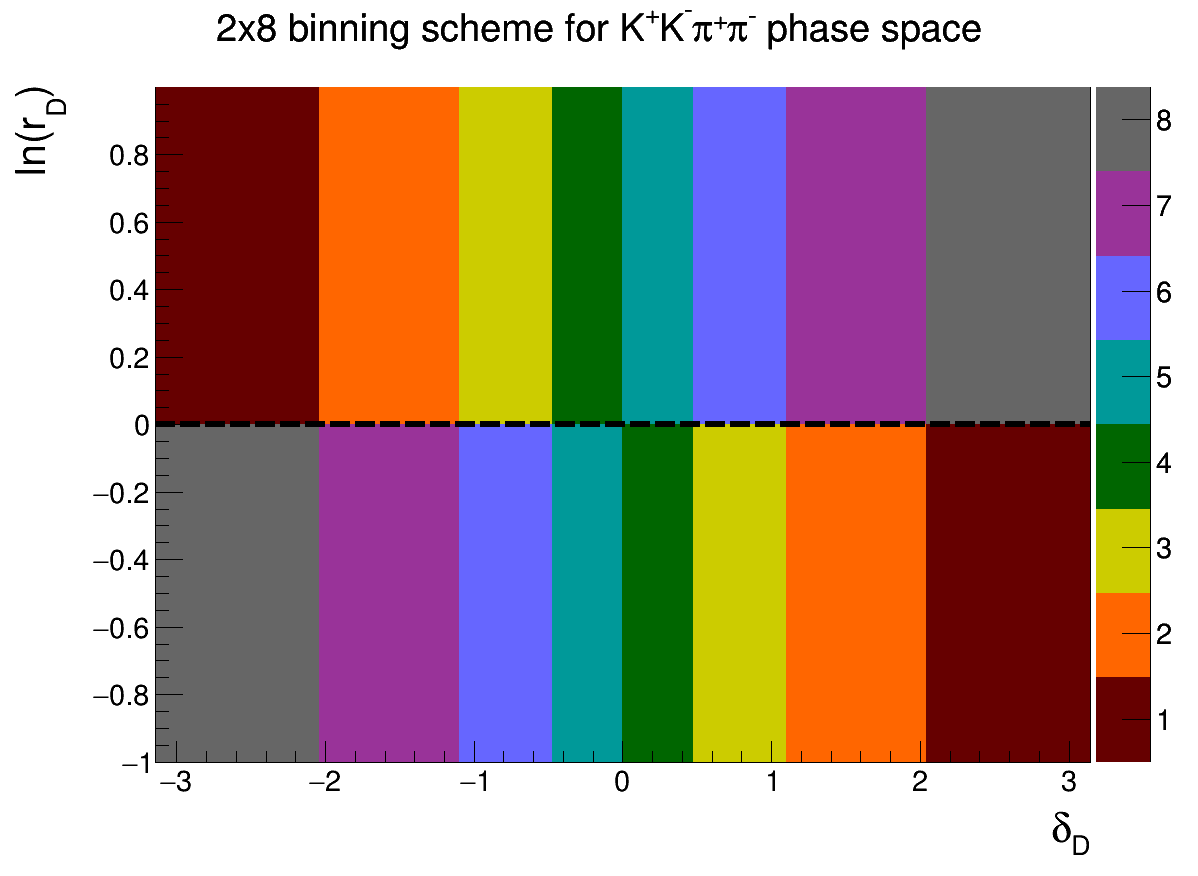
\includegraphics[width=1\textwidth]{Plots/BinningSchemePlot.png}
    \caption{Binning scheme definition for $2\times 8$ bins}
    \label{fig_binning_scheme}
  \end{subfigure}%
  \begin{subfigure}{0.5\textwidth}
    \centering
    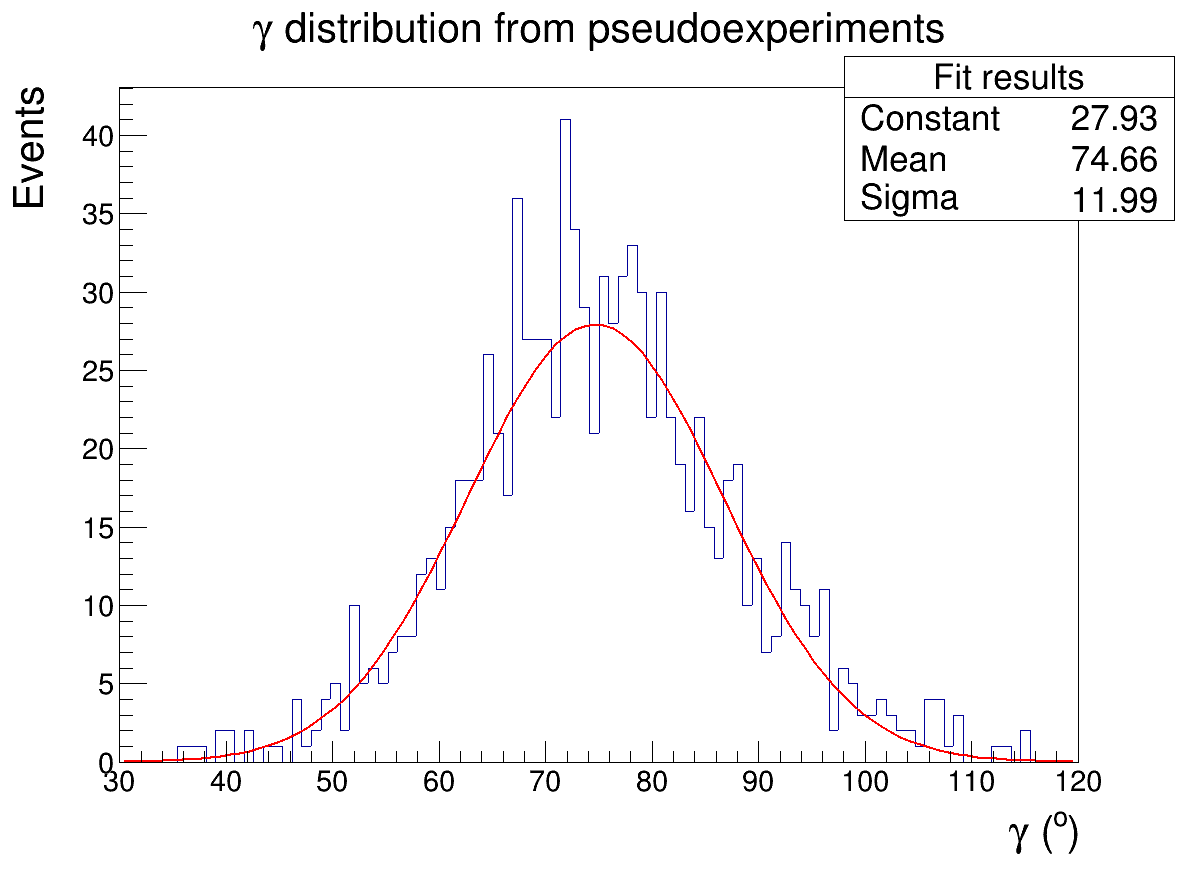
\includegraphics[width=1\textwidth]{Plots/GammaDistribution8BinsVariableWidth.png}
    \caption{Distribution of $\gamma$ from toy study}
    \label{fig_gamma_pull_study}
  \end{subfigure}
  \caption{}
\end{figure}

%%%%%%%%%%%%%%%%%%%%%%%%%%%%%%%%%%%%%%%%%%%%%%%%%%%%%%%%%%%%%%%
\section{\texorpdfstring{$B^\pm$}{B} candidate selection}
\subsection{Signal candidate requirements}
\noindent The $B^\pm\to Dh^\pm (h = \pi, K)$ candidates, with $D\to K^+K^-\pi^+\pi^-$, are reconstructed from five charged tracks. Currently, only Run $2$ data has been processed, but Run $1$ will be included later as well. The standard track and trigger requirements follow Ref. \cite{cite_LHCbGGSZKSpipi}. To ensure that $D$ is real, the $K^+K^-\pi^+\pi^-$ must be inside a $\SI{25}{\mega\eV}$ mass window of the $D^0$ PDG mass. Then the tracks are refitted with their invariant mass constrained to the $D^0$ mass and their momenta pointing to the primary vertex. A cut on the $\chi^2$ from this fit, at $\ln(\chi^2) < 3$, will remove most of the sidebands in the $D$ invariant mass.

A mutually exclusive Particle Identification (PID) cut separates the $B^\pm\to D\pi^\pm$ and $DK^\pm$ candidates. Moreover, the $K^\pm$ daughters from $D$ and the $h^\pm$ daughter from $B^\pm$ are required to have momentum $p < \SI{100}{\giga\eV}$, which is the optimal range for the RICH.

Sections \ref{subsection_BDT}-\ref{subsection_charmless_misID} discuss more specialized selections to remove specific backgrounds.

\subsection{Boosted Decision Tree}
\label{subsection_BDT}
\noindent A Boosted Decision Tree (BDT) was used to remove the combinatorial background, which is the largest background. The BDT was trained using Monte Carlo (MC) $B^\pm$ samples as a signal sample and the region $m(Dh^\pm)\in[5800, 7000]\si{\mega\eV}$ in data as a background sample. The training variables are similar to those in Ref. \cite{cite_LHCbGGSZKSpipi}. The input data was randomly split into equal training and test samples. After training, $99.4\%$ of the background was removed and $93\%$ of the signal remained in the test sample.

\subsection{Mis-ID and charmless backgrounds}
\label{subsection_charmless_misID}
\noindent A significant mis-ID background are $B^\pm\to Dh^\pm$ candidates where $D\to K^\pm\pi^\mp\pi^\pm\pi^\mp$ and a pion is assigned a kaon hypothesis. This is studied with MC samples. After reconstruction, the simulation indicate that $7.2\%$ of $B^\pm$ candidates inside the signal region are $D\to K^\pm\pi^\mp\pi^\pm\pi^\mp$. A tighter PID requirement reduces this fraction to $1.8\%$ while keeping $93\%$ of signal candidates.

Charmless backgrounds are $B^\pm$ candidates that decay into five charged particles without an intermediate $D$ meson. These candidates form a signal in the $B^\pm$ mass spectrum, but does not peak in the $D$ mass spectrum. The $D$ mass window removes some of this, but a large fraction remains under the $D$ peak.

To estimate the contamination, a selection was done without imposing a $\chi^2$ cut on the refitted $D$ daughters. This preserves the $D$ mass sidebands. A mass window in the lower sideband, $m(K^+K^-\pi^+\pi^-)\in[\SI{1770}{\mega\eV}, \SI{1820}{\mega\eV}]$ was selected. The $B^\pm$ mass spectrum is shown in Fig. \ref{fig_Bmass_charmless} for $B^\pm\to DK^\pm$ candidates.

\begin{figure}[H] 
  \centering
  \begin{subfigure}{0.5\textwidth}
    \centering
    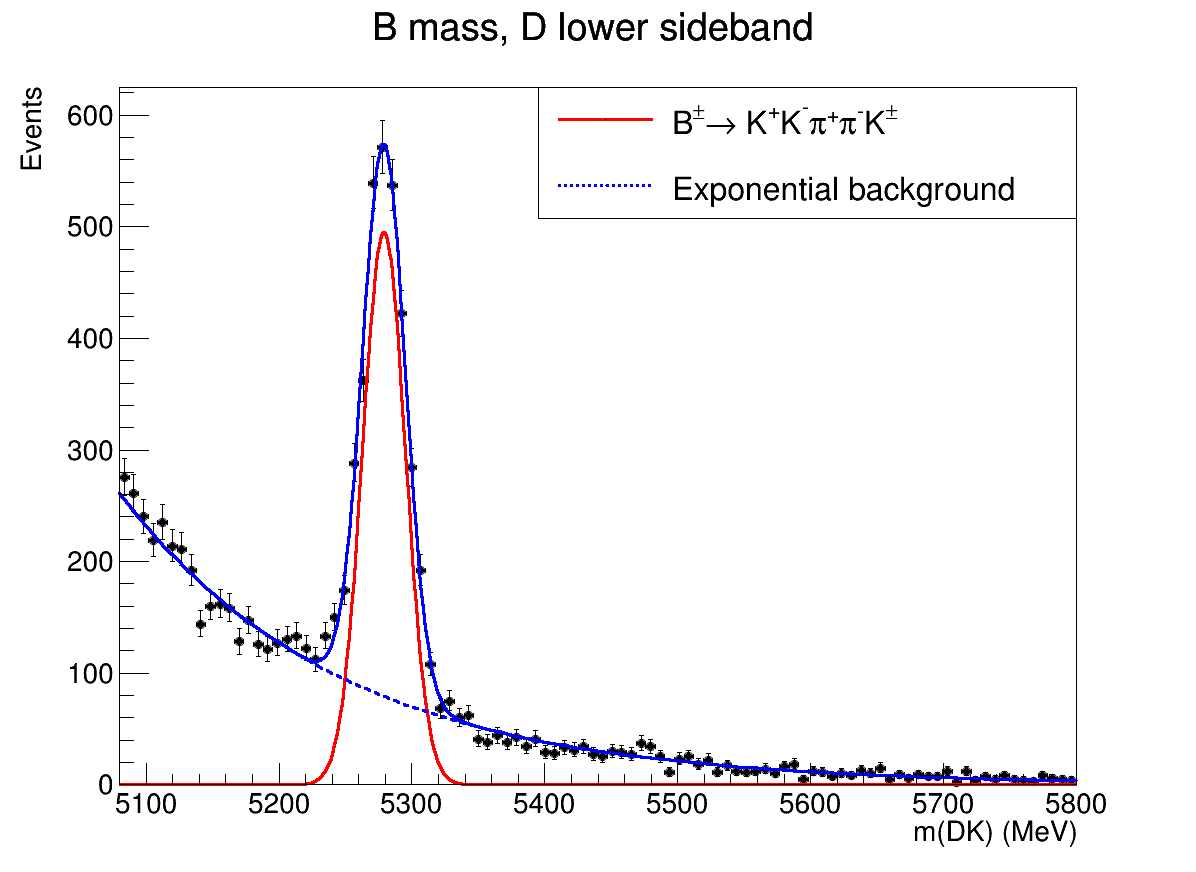
\includegraphics[width=1\textwidth]{Plots/B2DKLower_Charmless.png}
    \caption{The $B^\pm$ invariant mass in the $D$ invariant mass lower sideband.}
    \label{fig_Bmass_charmless}
  \end{subfigure}%
  \begin{subfigure}{0.5\textwidth}
    \centering
    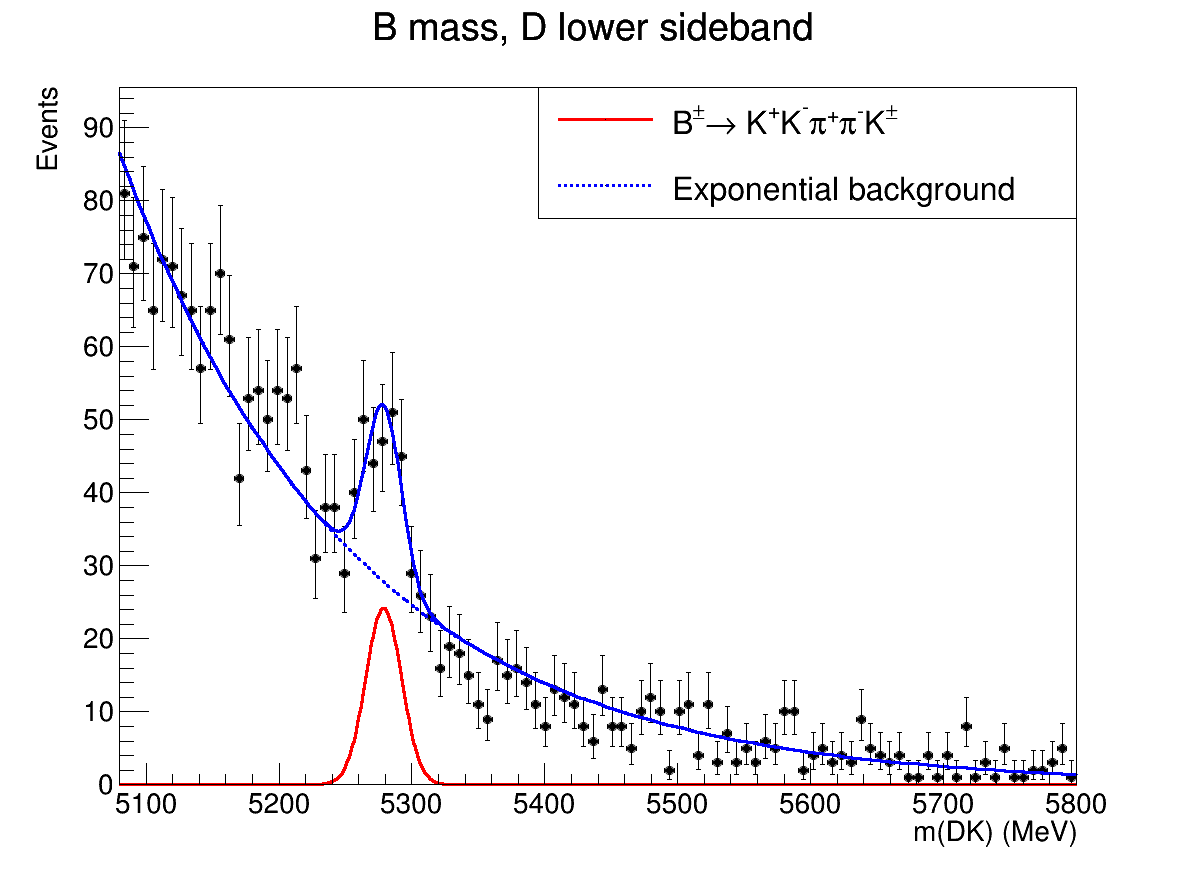
\includegraphics[width=1\textwidth]{Plots/B2DKLowerFDCut_Charmless.png}
    \caption{The $B^\pm$ invariant mass in the $D$ invariant mass lower sideband with a flight significance cut.}
    \label{fig_Bmass_charmless_fdcut}
  \end{subfigure}
  \caption{}
\end{figure}

A fit to Fig. \ref{fig_Bmass_charmless} with a Gaussian signal and an exponential background gives a yield of $\SI{2605(57)}{}$. A cut on the flight significance, defined as the flight distance divided by its error, reduces this yield to $\SI{110(19)}{}$, shown in Fig. \ref{fig_Bmass_charmless_fdcut}. No charmless peak was found in the corresponding $B^\pm\to D\pi^\pm$ invariant mass spectrum.

%%%%%%%%%%%%%%%%%%%%%%%%%%%%%%%%%%%%%%%%%%%%%%%%%%%%%%%%%%%%%%%
\section{Fit to extract CP observables}
\subsection{Global fit and invariant mass spectra}
\label{section_global_fit}
\noindent A global ML fit of all $B^\pm\to Dh^\pm (h = K, \pi)$ candidates was performed to determine yields and mass shape parameters in the $B^\pm$ mass spectrum, shown in Fig. \ref{fig_Bmass_Global}. The mass shape parameterizations and their parameters are taken from Ref. \cite{cite_LHCbGGSZKSpipi}. Minor adjustments are needed for the final analysis.

The combinatorial background is parameterized by an exponential function. The signal is a sum of a Gaussian $f_\text{G}(m|m_B, \sigma)$ and a modified Gaussian,

\begin{equation}
  f_\text{MG}(m|m_B, \sigma, \alpha_L, \alpha_R, \beta)\propto
  \begin{cases}
    \exp\Big(\frac{-\Delta m^2(1 + \beta\Delta m^2)}{2\sigma^2 + \alpha_L\Delta m^2}\Big), \Delta m = m - m_B < 0 \\
    \exp\Big(\frac{-\Delta m^2(1 + \beta\Delta m^2)}{2\sigma^2 + \alpha_R\Delta m^2}\Big), \Delta m = m - m_B > 0 \\
  \end{cases},
\end{equation}
which accounts for the radiated tail and wider resolution. To the left of the $B^\pm$ mass peak are contributions from partially reconstructed backgrounds. These are mainly $B^\pm$ or $B^0$ decays to $Dh^\pm\pi$ or $D^*h^\pm$ with $D^*\to D\pi$ or $D^*\to D\gamma$. The missing pion or photon leads to peaking at lower mass. Furthermore, in the $B^\pm\to DK^\pm$ channel on the right of the signal, there is a mis-ID component of $B^\pm\to D\pi^\pm$ candidates, where the $\pi^\pm$ is identified as $K^\pm$. This channel also has a component of $B_s\to DK^\pm\pi^\mp$ with a missing pion, and a component of partially reconstructed background from $B^\pm$ and $B^0$ candidates where the $\pi^\pm$ daughter is mis-identified as a $K^\pm$. The PDF shapes of the partially reconstructed background at low mass is described in Ref. \cite{cite_LHCbGGSZKSpipi}. The fitted yield of $B^\pm\to DK^\pm$ and $B^\pm\to D\pi^\pm$ candidates are $\SI{2290(59)}{}$ and $\SI{33113(211)}{}$, respectively.

\begin{figure}[H] 
  \centering
  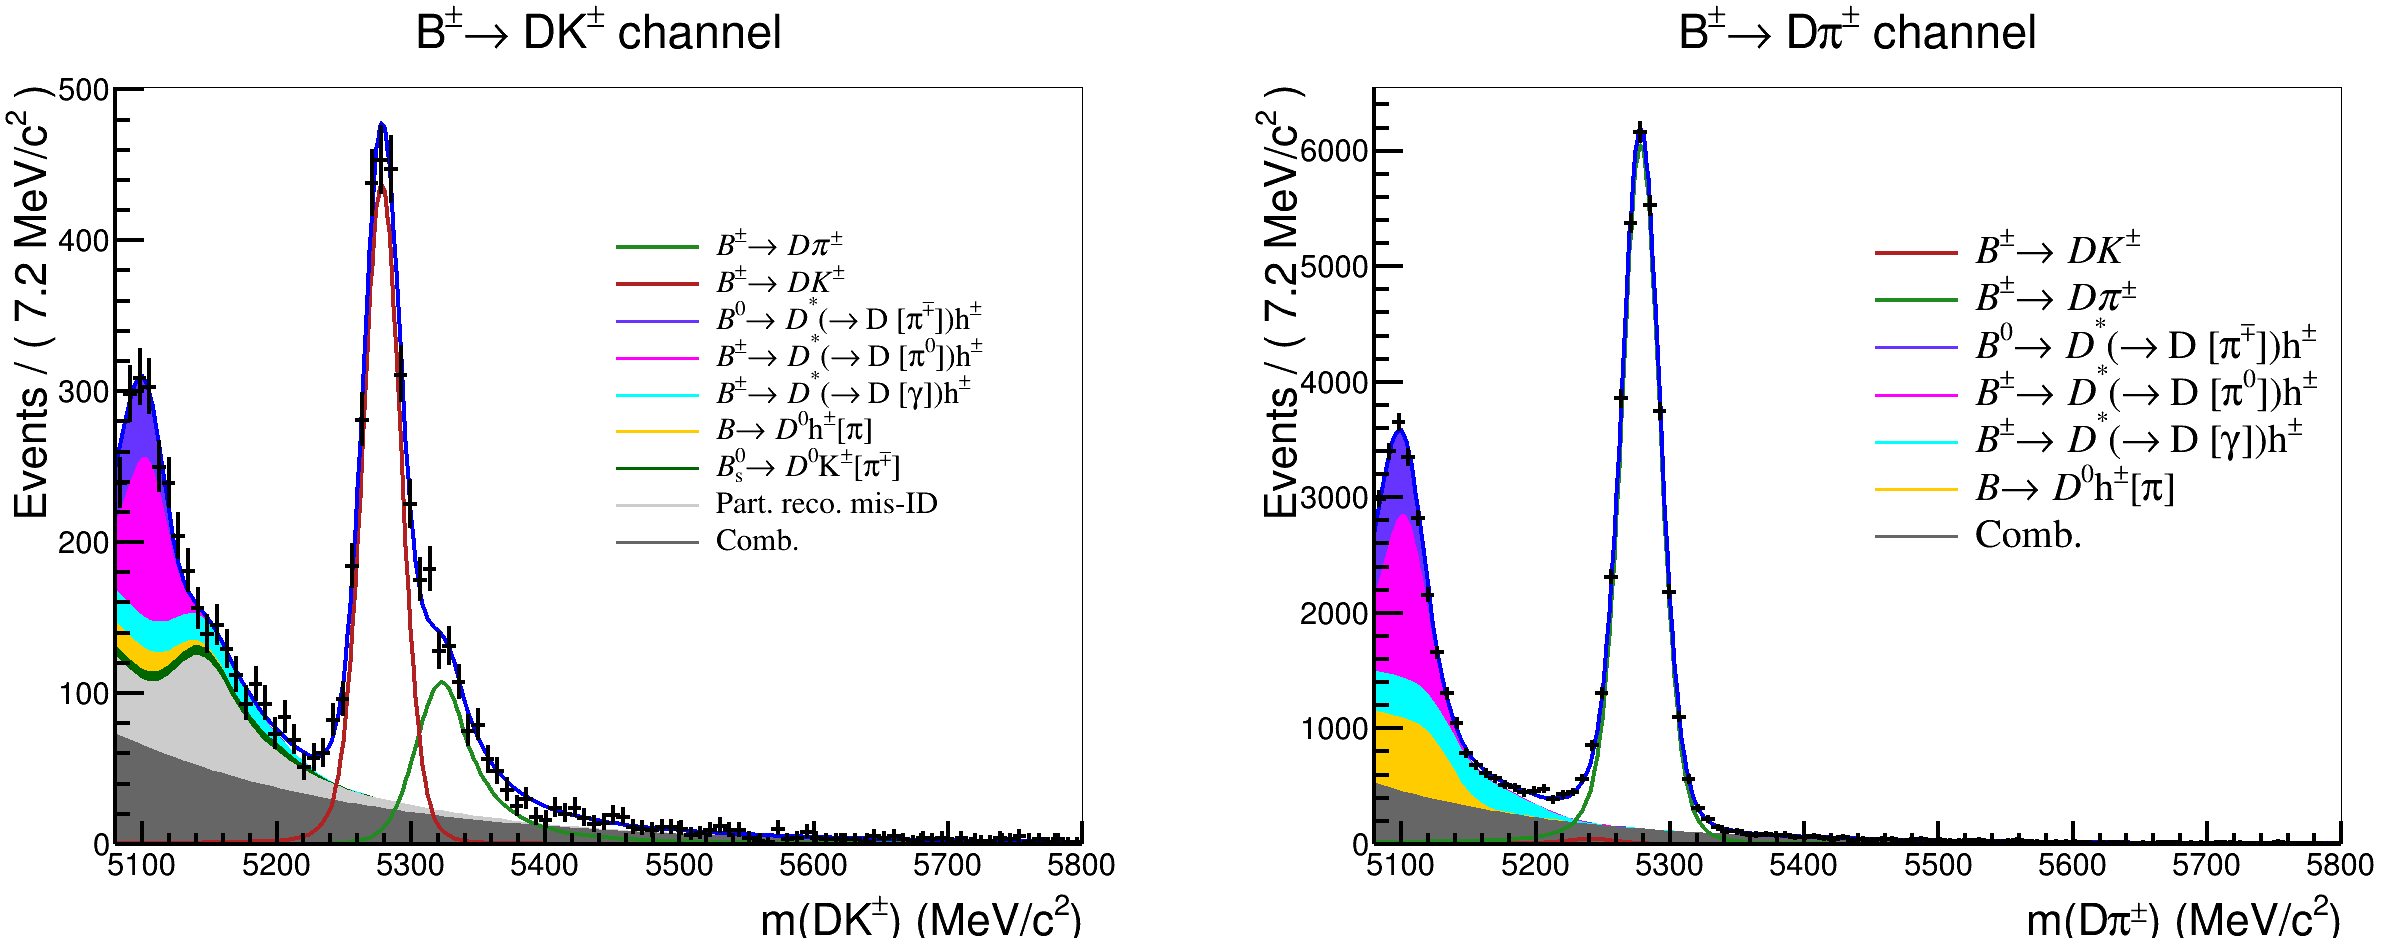
\includegraphics[width=1\textwidth]{Plots/GlobalFit.png}
  \caption{Global mass fit of $B^\pm\to DK^\pm$ (left) and $B^\pm\to D\pi^\pm$ (right).}
  \label{fig_Bmass_Global}
\end{figure}

\subsection{Binned CP fit and CP observables}
\noindent After the global fit, $B^\pm$ candidates are split by charge and bins, using the binning scheme from Section \ref{section_binning_scheme}. A simultaneous ML fit is performed, with shape parameters from the global fit fixed. The yield of signal, partially reconstructed background and combinatorial background in each bin are floated.

The fitted CP observables are shown in Figs. \ref{fig_xpm_ypm}-\ref{fig_xxi_yxi}, and they may be interpreted in terms of $\gamma$, $\delta_B^{DK}$, $r_B^{DK}$, $\delta^{D\pi}$ and $r_B^{D\pi}$. However, this step is only performed at the end to avoid any human bias in the final result. Geometrically, the angle between $(x_+^{DK}, y_+^{DK})$ and $(x_-^{DK}, y_-^{DK})$ is $2\gamma$.

To check the fit robustness, $1000$ toy datasets are generated, with both global and CP fit, using the fitted parameters. Each toy datasets is then run through the same fitting procecure and the pull distibutions of each floated variable is checked. It was found that all CP observables have pulls with zero mean and unit standard deviation. Two global fit parameters had slightly underestimated errors which can be accounted for.

\begin{figure}[H] 
  \centering
  \begin{subfigure}{0.5\textwidth}
    \centering
    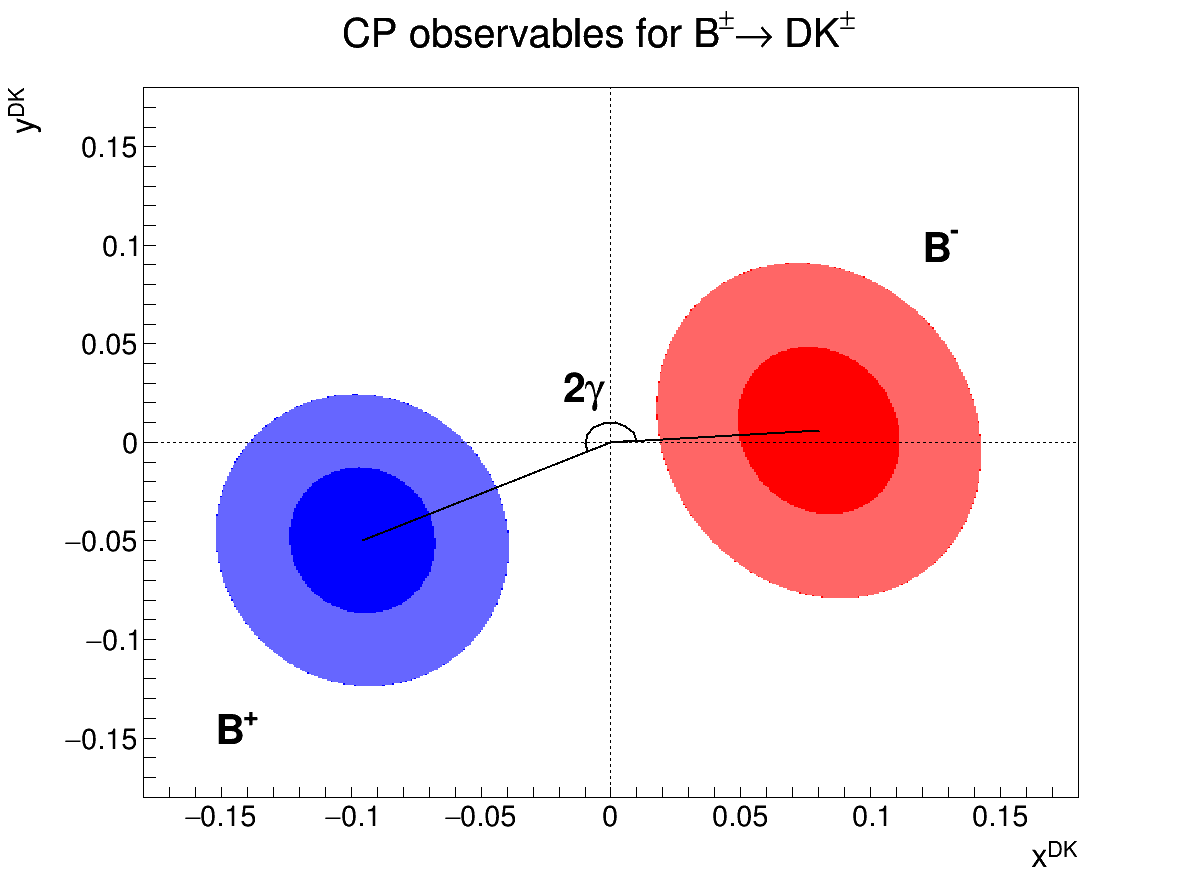
\includegraphics[width=1\textwidth]{Plots/CPContours.png}
    \caption{Confidence levels at $68.2\%$ and $95.5\%$ of $(x_+^{DK}, y_+^{DK})$ and $(x_-^{DK}, y_-^{DK})$.}
    \label{fig_xpm_ypm}
  \end{subfigure}%
  \begin{subfigure}{0.5\textwidth}
    \centering
    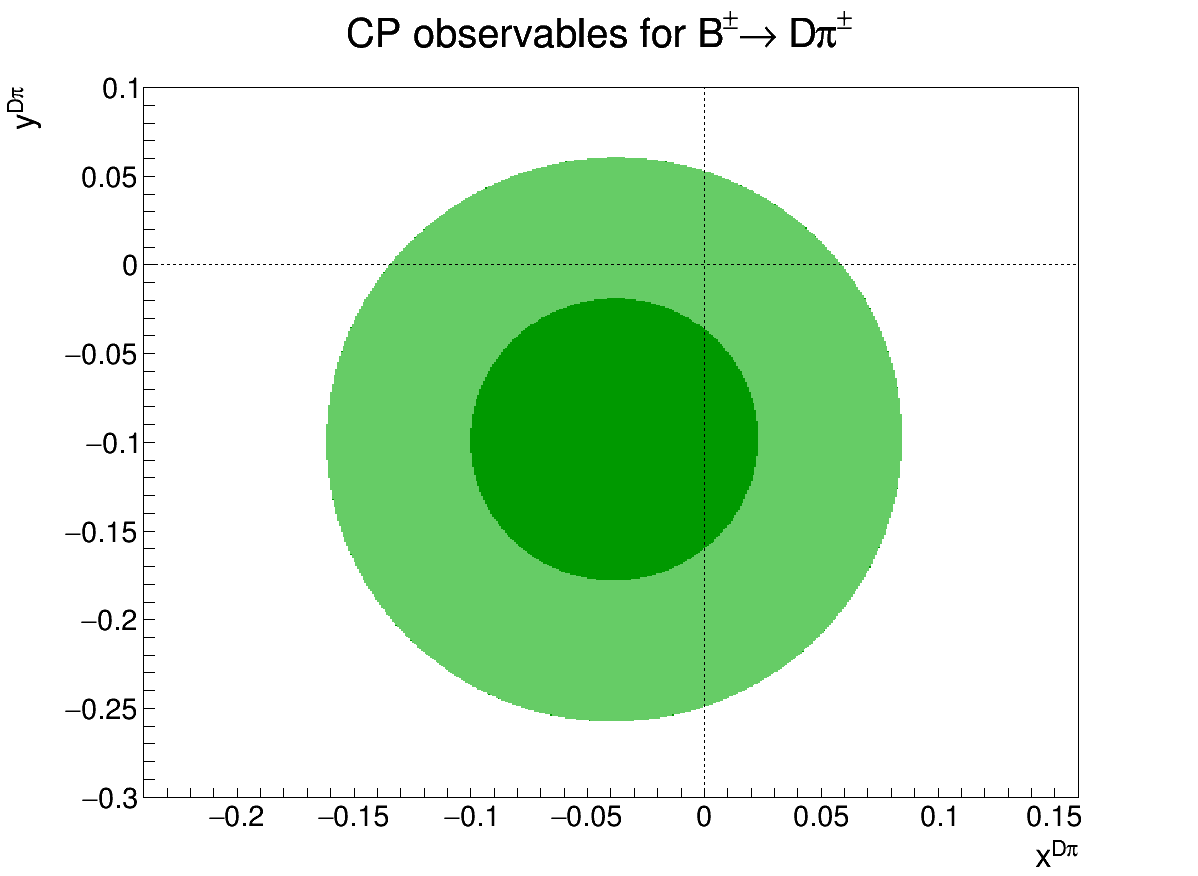
\includegraphics[width=1\textwidth]{Plots/CPXiContours.png}
  \caption{Confidence levels at $68.2\%$ and $95.5\%$ of $(x_\xi^{D\pi}, y_\xi^{D\pi})$.}
    \label{fig_xxi_yxi}
  \end{subfigure}
\end{figure}

%%%%%%%%%%%%%%%%%%%%%%%%%%%%%%%%%%%%%%%%%%%%%%%%%%%%%%%%%%%%%%%
\section{External strong phase input from BESIII}
\noindent The reconstruction of charged and neutral particles in BESIII data follows a similar strategy to Ref. \cite{cite_KSKKAnalysis}. The aim is to obtain the single and double tagged event yields. Peaking backgrounds are accounted for using the inclusive MC samples. The yields are used in a ML fit of Eqs. \eqref{eq_Mi}-\eqref{eq_Mij} to obtain $c_i$ and $s_i$.

Since the beams are symmetric, each $D$ meson has energy $E_\text{beam}$. For each $D$ meson, the energy difference $\Delta E$ and beam-constrained mass $M_\text{BC}$ may be defined as

\begin{equation*}
  \Delta E = \sum_i E_i - E_\text{beam}, \quad M_\text{BC} = \sqrt{E_\text{beam}^2 - \abs{\sum_i\vb{p}_i}^2},
\end{equation*}
where the sum runs over all $D$ daughters. For a perfectly reconstructed $D$ meson, $\Delta E = 0$, but the peak is broadened by detector resolution. In tag modes with showers, the $\Delta E$ distribution has a left tail due to energy leakage through the calorimeter. The beam-constrained mass is the $D$ invariant mass, but using the more accurate beam energy.

In single tagged events, a mode-dependent cut on $\Delta E$ is chosen by fitting a double Gaussian for the signal peak and a second order polynomial for the background. A cut around $\pm 3\sigma$ removes some combinatorial background. For modes with photon showers, the left cut is extended to $-4\sigma$.

The single tag yield is obtained from a ML fit of the $M_\text{BC}$ distribution. An Argus shape parameterizes the continuous combinatorial background. The signal shape is taken from an exclusive MC sample convolved with a Gaussian. Peaking backgrounds, if present, are accounted for with Gaussian shapes. An example of such a fit, for $D\to K^+K^-\pi^+\pi^-$ is shown in Fig. \ref{fig_styield}, where the largest peaking background is $D\to K_S^0K^+K^-$.

In double tagged events, the same cuts on $\Delta E$ used for single tagged events are applied. Fig. \ref{fig_dtyield} shows double tagged $D\to K^+K^-\pi^+\pi^-$ versus $D\to K^\pm\pi^\mp$, where the beam constrained mass for both $D$ mesons are plotted in a $2$D scatter plot.

A sideband subtraction technique is used to obtain the yield. In Fig. \ref{fig_dtyield}, region $S$ is the signal region, while $A$ and $B$ are events where only one $D$ meson is real. Region $C$ are events where daughters tracks have been swapped between the $D$ mesons. Region $D$ contains non-charm  combinatorial background. The total background is estimated using

\begin{equation*}
  B = P + \frac{a_S}{a_D}Y_D + \sum_{i = A, B, C}\frac{a_S}{a_i}\Big(Y_i - \frac{a_i}{A_D}Y_D\Big),
\end{equation*}
where $P$ is the peaking background found from inclusive MC, $Y_i$ is the yield in region $i$ and $a_i$ is the corresponding area of the region.

\begin{figure}[H] 
  \centering
  \begin{subfigure}{0.5\textwidth}
    \centering
    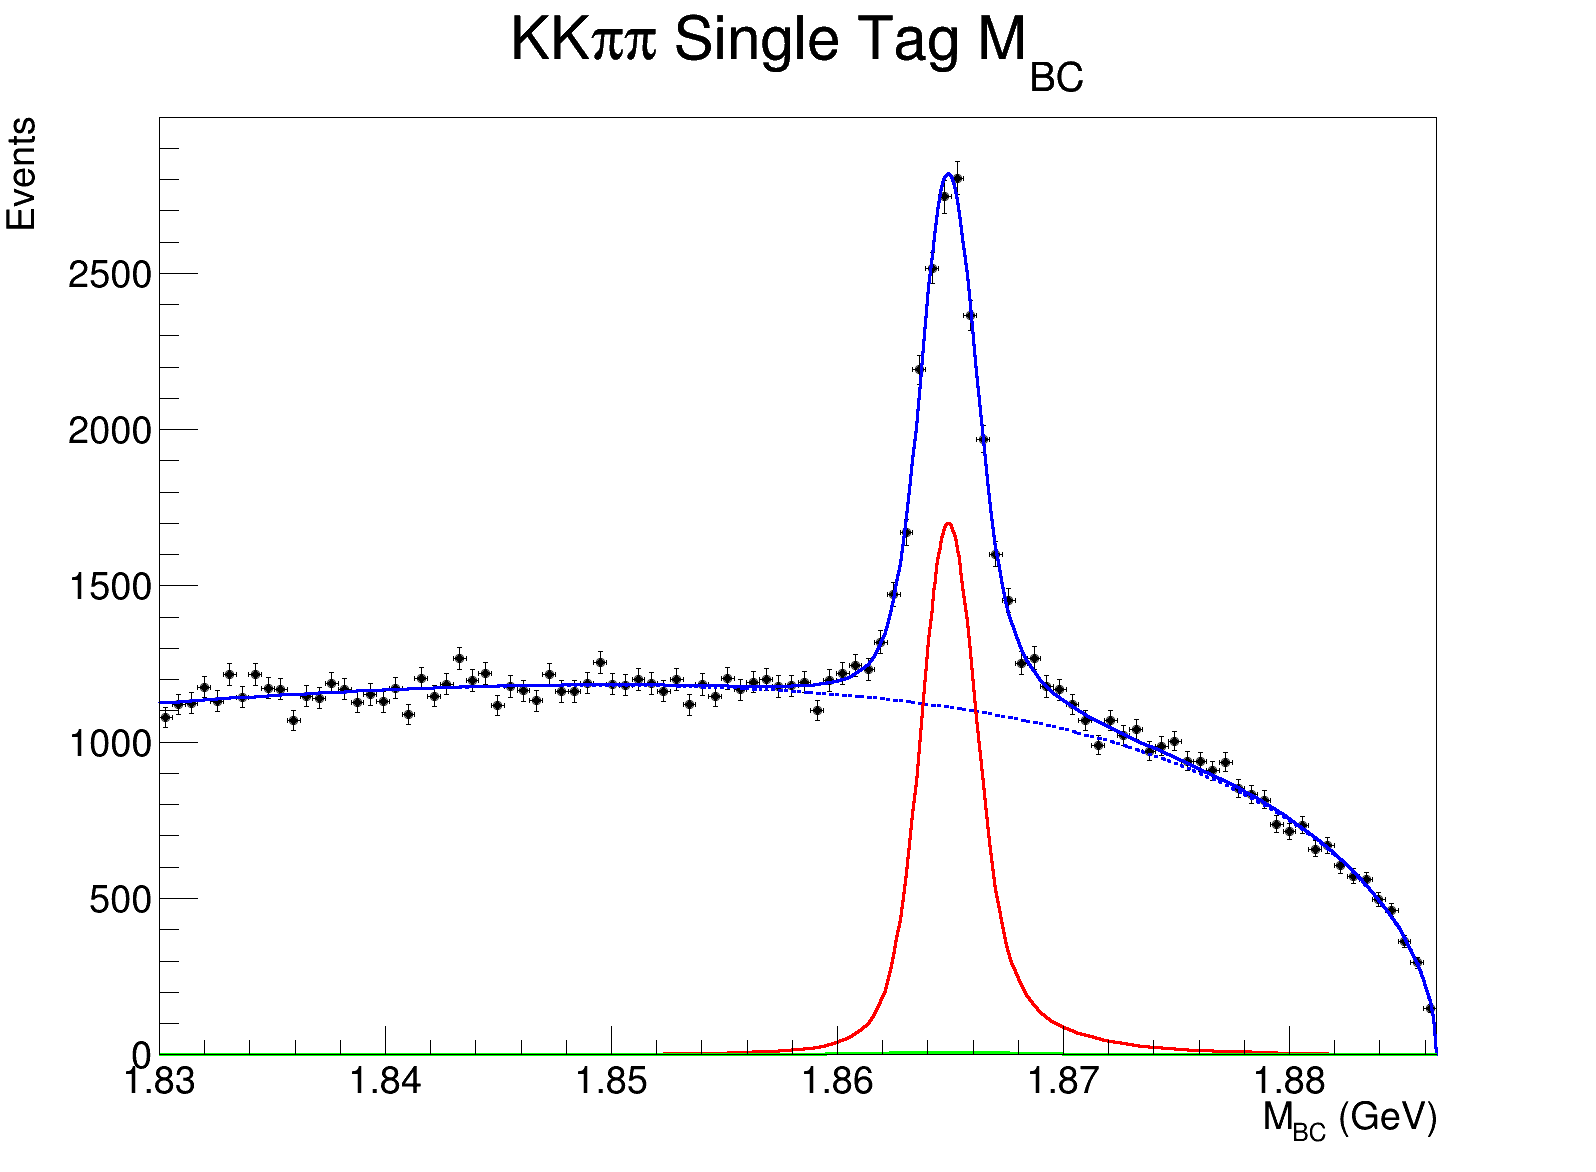
\includegraphics[width=1\textwidth]{Plots/KKpipiSingleTagMBCPlot.png}
    \caption{Fit of single tagged $M_\text{BC}$ distribution to obtain single tag yields.}
    \label{fig_styield}
  \end{subfigure}%
  \begin{subfigure}{0.5\textwidth}
    \centering
    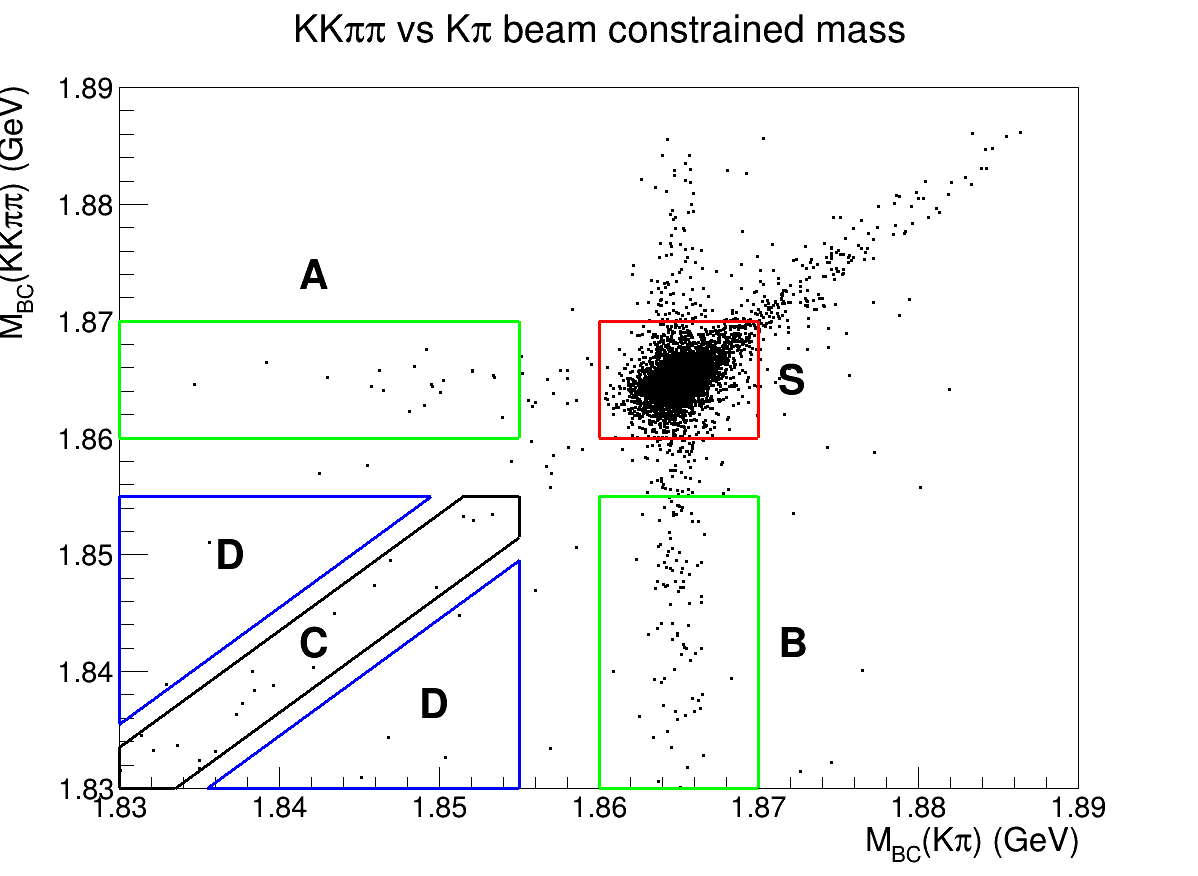
\includegraphics[width=1\textwidth]{Plots/KpiDoubleTagYield.png}
  \caption{Background subtraction technique of double tagged $M_\text{BC}$ distributions to obtain double tag yields}
    \label{fig_dtyield}
  \end{subfigure}
  \caption{}
\end{figure}

It is useful to compare the yields with the prediction from the LHCb model. In Fig. \ref{fig_flavour_yield}, $D\to K^\pm\pi^\mp$ vs $D\to K^+K^-\pi^+\pi^-$ events are shown (data points), with the amplitude model prediction (solid line), using $2\times 4$ bins. Fig. \ref{fig_cp_yield} shows $D\to K^+K^-\pi^+\pi^-$ events, tagged with a CP even tag mode $D\to K^+K^-$ and a CP odd tag mode $K_S^0\pi^0$, without binning. Both plots are normalized by the $K^\pm\pi^\mp$ yields. The LHCb model agrees reasonably well with the BESIII data. However, the yields have not been corrected for efficiency or bin migration effects, and a perfect agreement is therefore not expected.

\begin{figure}[H] 
  \centering
  \begin{subfigure}{0.5\textwidth}
    \centering
    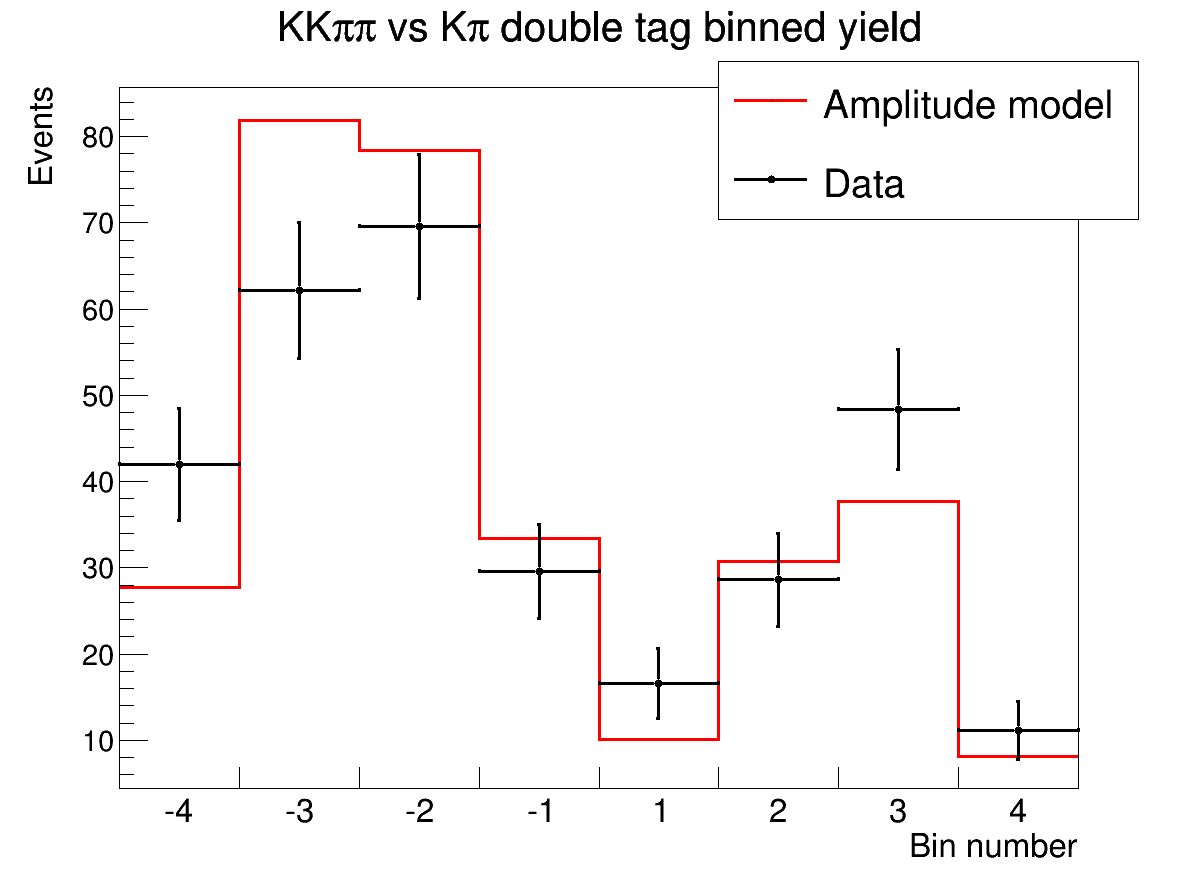
\includegraphics[width=1\textwidth]{Plots/DoubleTagYieldFlavour.png}
    \caption{Binned double tag yield of $K^+K^-\pi^+\pi^-$ versus $K^\pm\pi^\mp$ events.}
    \label{fig_flavour_yield}
  \end{subfigure}%
  \begin{subfigure}{0.5\textwidth}
    \centering
    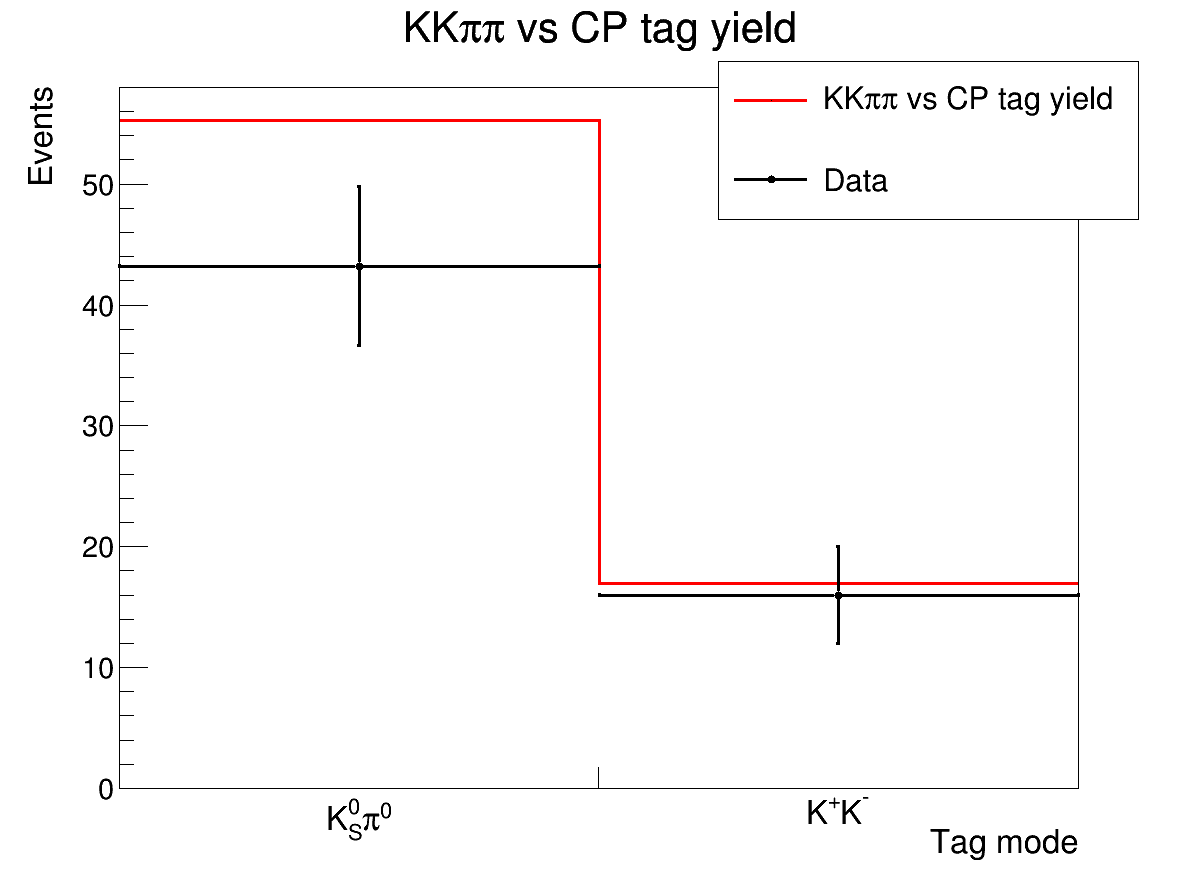
\includegraphics[width=1\textwidth]{Plots/DoubleTagYieldInclusiveCP.png}
  \caption{Inclusive double tag yield of $K^+K^-\pi^+\pi^-$ versus $K^+K^-$ and $K_S^0\pi^0$ events.}
    \label{fig_cp_yield}
  \end{subfigure}
\end{figure}

%%%%%%%%%%%%%%%%%%%%%%%%%%%%%%%%%%%%%%%%%%%%%%%%%%%%%%%%%%%%%%%
\section{Discussion of future work}
\noindent Discuss the future plans with Guy first!


%%%%%%%%%%%%%%%%%%%%%%%%%%%%%%%%%%%%%%%%%%%%%%%%%%%%%%%%%%%%%%%                                                                          
\bibliography{references}
\bibliographystyle{unsrt}

%%%%%%%%%%%%%%%%%%%%%%%%%%%%%%%%%%%%%%%%%%%%%%%%%%%%%%%%%%%%%%%
\newpage
\section{DPhil thesis plan}
\noindent Discuss DPhil thesis plan with Guy first!

\end{document}